\chapter{Controllo dei Robot}

Questo capitolo tratta tutte le nozioni e accorgimenti utillizzati per la creazione del nodo di comunicazione con i robot e-Puck
\section{Comunicazione}
	Come gi\`a anticipato nel capitolo precedente, la comunicazione con i robot avviene tramite una connessione seriale virtuale attraverso la quale vengono scambiati messaggi sotto forma di array di caratteri.
	
	Il firmware precaricato negli e-Puck fornisce una modalit\`a di interazione tramite connessione seriale nella quale \`e possibile accedere ai valori misurati da tutti i sensori e impartire vari comandi.
	In particolare inviando ``D,\emph{fl},\emph{fr}\textbackslash n'' \`e possibile impostare la frequenza di passo dei motori sinistro e destro rispettivamente ai valori di \emph{fl} e \emph{fr}.
	I valori accettabili per le due frequenze sono i numeri interi compresi tra -1000 e 1000, frequenze alle quali corrisponde una rotazione completa indietro o avanti della ruota in un secondo.
	
	  
\section{Modellizzazione}
	I robot utilizzati possono essere classificati come dei monocicli ad azionamento differenziale, l'assenza di una rotella di suppporto non crea problemi in quanto lo scheletro del robot permette la stabilit\`a e consente il movimento.
	\begin{figure}[H]
	\centering
	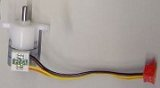
\includegraphics[width=4cm]{images/motor+cable}
	\caption{Modello schematico di un monociclo ad azionamento differenziale \label{unicycle}}
	\end{figure}
	
	Secondo questo modello il robot pu\`o avere due distinte componenti di velocit\`a: una di traslazione \emph{v}, ortogonale all'asse delle due ruote e parallela al piano di spostamento, e una di rotazione $\omega$ ortogonale al piano di spostamento del robot nel punto medio della distanza tra le due ruote.
	
	Da \emph{v} e $\omega$ possono essere stabilite le velocit\`a da assegnare alle singole ruote $\omega$r e $\omega$l tramite le seguenti relazioni in cui r \`e il raggio delle ruote e d la distanza tra i centri delle ruote:
	
	\begin{center}		
	\begin{tabular}{ccc}
			$\bigg \{
				\begin{array}{r}
				v=\frac{(\omega r+\omega l)r}{2}\\
				\omega = \frac{(\omega r-\omega l)r}{d}\\
				\end{array}$ 
 	& $\to$
 	&$\bigg \{
 		\begin{array}{r}
 		\omega r=\frac{2\emph{v}+d\omega }{r}\\
 		\omega l= \frac{2\emph{v}-d\omega}{r}\\
 		\end{array}$   \\ 
	\end{tabular} 
	\end{center}
	
	
	Per ricavare la frequenza di passo delle ruote si moltiplica i valori ottenuti per  $\frac{1000}{2\pi}$ che corrisponde al rapporto tra il numero di passi necessari per compiere una rotazione completa della ruota e una rotazione completa in radanti.
	
	\begin{center}	
	$\begin{array}{r}
	 		fr=\frac{1000}{2\pi}\times \omega r\\ 
	 		fl= \frac{1000}{2\pi}\times \omega l\\
	 		\end{array}$
	\end{center}
	
	Il nodo realizzato dunque riceve un messaggio tramite topic contenente \emph{v} e $\omega$ e ricava le frequenze di passo da assegnare alle ruote.
	Questi valori sono inviati al robot tramite connessione seriale utilizzando il messaggio descritto nella sezione precedente.
	Inoltre se il nodo non riceve messaggi di velocit\`a per due secondi invia al robot un comando per fermare le ruote ovvero imposta la frequenza di passo delle ruote a 0.
	
\section{Accorgimenti}
	Per evitare eventuali problemi di connessione e assicurare che le connessioni siano ripartite correttamente tra i due adatatori Bluetooth \`e stato creato uno script con linguaggio bash che utilizza i comandi ``rfcomm release'' e ``rfcomm bind'' per associare a ogni adattatore quattro robot tramite gli indirizzi MAC dei vari dispositivi.
	Lo script viene lanciato digitando ``./epuckbtset.sh'' in un terminale che punta alla cartella contenente il file bash.
	 	
	


